%
% einleitung.tex -- Beispiel-File für die Einleitung
%
% (c) 2020 Prof Dr Andreas Müller, Hochschule Rapperswil
%%
\section{Teil 0\label{erdbeben:section:teil0}}
\rhead{Erdbeben}
\section{Erdbebenmessung}
\subsection{Was ist ein Erdbeben}
Fabio
\subsection{Funktion eines Seismograph}
Um ein Erdbeben kenntlich zu machen, werden in der Regel Seismographen mit vielen Sensoren verwendet. 
Ein Seismograph besteht im Grunde aus einer federgelagerten Masse. Wirkt eine Bodenerregung auf das Gerät ein, bleibt die gekoppelte Masse stehen aber das Gehäuse schwingt mit.
Relativbewegung des Bodens kann damit als Auslenkung im Zeitverlauf gemessen werden.
In modernen Seismographen wird die Bodenbewegung in alle Richtungen gemessen, sowohl Horizontal als auch Vertikal. 
Wir konstruieren uns eine einfachere Version eines Seismographen mit eine Gehäuse, an dem zwei Federn und eine Masse befestigt ist. 
Ein Sensor unter der Masse misst die Position, bzw. die Auslenkung der Feder und der Masse.
Dies bedeutet unser Seismograph kann nur in eine Dimension Messwerte aufnehmen. 

\begin{figure}
 \begin{center}
 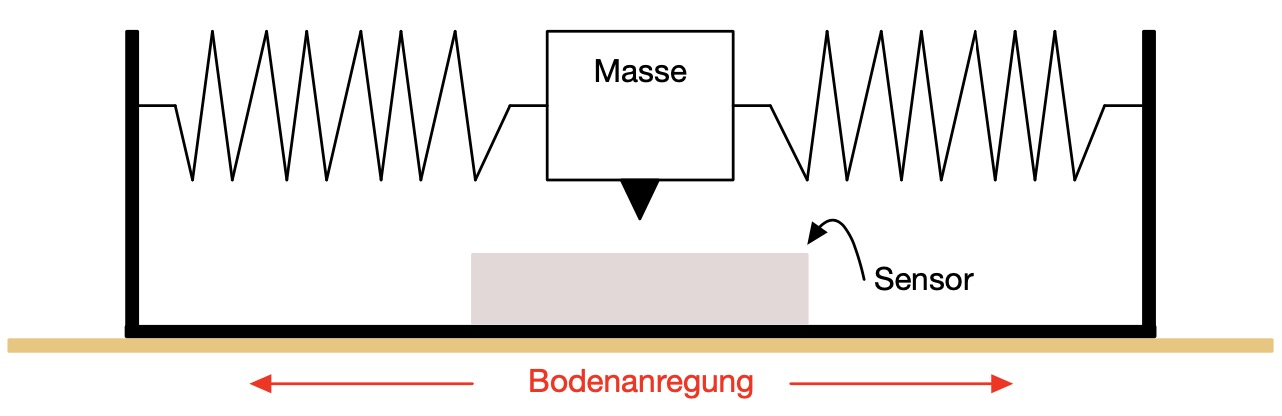
\includegraphics[width=5cm]{papers/erdbeben/Apperatur}
 \caption{Aufbau des Seismographen mit Gehäuse, Masse, Federn und Sensor}
 \end{center}
\end{figure}

\subsection{Ziel}
Unser Seismograph misst nur die Position der Masse über die Zeit. 
Wir wollen jedoch die Beschleunigung $a(t)$ des Boden bzw. die Kraft $f(t)$ welche auf das Gehäuse wirkt bestimmten.  
Anhand dieser Beschleunigung bzw. der Krafteinwirkung durch die Bodenbewegung wird später das Bauwerk bemessen.
Dies bedeutet, die für uns interessante Grösse $f(t)$ wird nicht durch einen Sensor erfasst. 
Jedoch können wir durch zweifaches ableiten der Positionsmessung $s(t)$ die Beschleunigung der Masse berechnen. 
Das heisst: Die Messung ist zweifach Integriert die Kraft $f(t)$ + der Eigendynamik der Masse.
Um die Bewegung der Masse zu berechnen, müssen wir Gleichungen für unser System finden.

\subsection{Systemgleichung}
Im Fall unseres Seismographen, kann die Differentialgleichung zweiter Ordnung einer gedämpften Schwingung am harmonischen Oszillator verwendet werden. 
Diese lautet:
\begin{equation}
m\ddot s + 2k \dot s + Ds = f
\end{equation}
mit den Konstanten $m$ = Masse, $k$ = Dämpfungskonstante und $D$  = Federkonstante.
Um diese nun in die Systemmatrix umzuwandeln, wird die Differentialgleichung zweiter Ordnung substituiert:
\[ {x_1}=s \qquad
{x_2}=\dot s,  \qquad\]
Somit entstehen die Gleichungenür die Position $s(t)$ der Masse :
\[ \dot {x_1} = {x_2}\] 
und
\[ \dot x_2 = -\frac{D}{m} {x_1} -\frac{2k}{m} {x_2} + \frac{f} {m} \] für die Geschwindigkeit $v(t)$ der Masse.

Diese können wir nun in der Form
\[ {x_3}=-\frac{D}{m} {s_1} -\frac{2k}{m} {s_2} + \frac{f} {m} \]
auch als Matrix-Vektor-Gleichung darstellen.
Dafür wird die Gleichung in die Zustände aufgeteilt. 
Die für uns relevanten Zustände sind die Position der Masse, die Geschwindigkeit der Masse und die äussere Beschleunigung des ganzen System. 
Dabei muss unterschieden werden, um welche Beschleunigung es sich handelt. 
Das System beinhaltet sowohl eine Beschleunigung der Masse (innere Beschleunigung), als auch eine Beschleunigung der ganzen Apparatur (äussere Beschleunigung). 
In unserem Fall wird die äusseren Beschleunigung gesucht, da diese der Erdbebenanregung gleich kommt. 
\begin{equation}
\frac{d}{dt} \left(\begin{array}{c} {s_1} \\ {s_2}  \end{array}\right) = \left(
 \begin{array}{ccc} 	
0 & 1& 0 \\ 
- \frac{D}{m} &-\frac{2k}{m} & \frac{1} {m}\\
\end{array}\right)  \left(\begin{array}{c} {s_1} \\ {s_2} \\ {s_3} \end{array}\right).
\end{equation}

Durch Rücksubstituion ergibt sich:
\begin{equation}
\frac{d}{dt} \left(\begin{array}{c} s(t) \\ v(t) \end{array}\right) = \left(
 \begin{array}{ccc} 	
0 & 1& 0 \\ 
- \frac{D}{m} &-\frac{2k}{m} & \frac{1} {m}\\
\end{array}\right)  \left(\begin{array}{c} s(t)\\ v(t)\\ f(t) \end{array}\right).
\end{equation}
Wir wissen nicht wie sich die Kraft verhält. 
Deshalb treffen wir die Annahme, das sich die Kraft über die Beobachtungszeit nicht verändert. 
Diese unzutreffende Annahme wird später durch einen grossen Systemfehler kompensiert. 
Da die Kraft unbekannt ist, wird die letzte Zeile mit Nullen gefüllt, denn genau diese Werte wollen wir. 











